\DiaryEntry{Binomal Coefficients, Part I}{2015-10-28}{Combinatorics}

\subsection{Introduction}

A sequence (with non-repeating elements) depends on the order of its elements; whereas a set does not. The sequences $(1,2,3)$ and $(3,2,1)$ are therefore \textbf{different}; whereas the sets $\{1,2,3\}$ and $\{3,2,1\}$ are \textbf{equivalent}.

If we have a set of $n$ elements, we can generate $(n(n-1)\cdots(n-k+1)$) sequences of length $k$: There are $n$ possibilities for the first slot, $n-1$ possibilities for the second slot and so on. For the k-th slot (the last one), there are therefore $n-k+1$ possibilities left.

If we are interested in the number of sets, we need a relation between the number of different sequences and the number of different sets. A set with $k$ elements yields $k!$ different sequences. Therefore if we have a set of $n$ elements and we want to know how many sets of size $k$ we can build out of it, we have

\begin{equation}
\frac{n(n-1)\cdots(n-k+1)}{k!} = \frac{n!}{(n-k)!k!} = {n \choose k}
\end{equation}

possibilities.

\subsubsection{Example}

Consider the set $(\mathcal{S} =
\{1,2,3,4\}$) with $(n=4$)
and list all six 2-element subsets:

\[(1,2), (1,3), (1,4), (2,3), (2,4), (3,4)\]

We have ${4 \choose 2} = \frac{4 \cdot 3}{1 \cdot 2} = 6$. If we consider sequences instead, we have the following 2-element sequences:

\[(1,2), (1,3), (1,4), (2,1), (2,3), (2,4), (3,1), (3,2), (3,4), (4,1), (4,2), (4,3)\]

Note that e.g.~the sequences $(1,2)$) and $(2,1)$) are \textbf{not} equivalent and therefore counted separately. There are $(4 \cdot 3 = 12$) such subsequences. If we finally allow duplicate elements in the sequences, then we obtain the following

\[ (1,1), (1,2), (1,3), (1,4), (2,1), (2,2), (2,3), (2,4), (3,1), (3,2), (3,3), (3,4), (4,1), (4,2), (4,3), (4,4) \]

There are $n^k = 4^2 = 16$ such sequences.

\subsection{Identities}

Table of the binomial coefficients:

\begin{figure}[H]
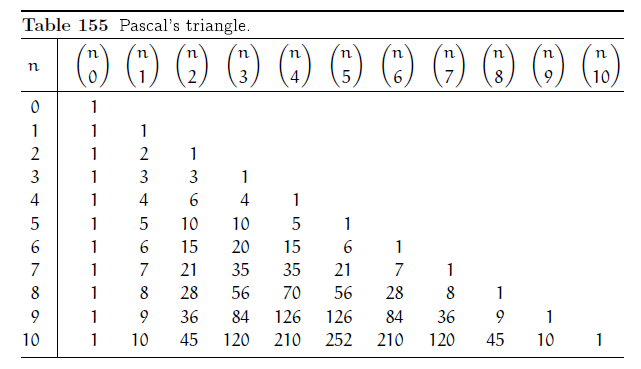
\includegraphics[scale=0.7]{images/binomials_01.png}
\end{figure}

We see that

\[ {n \choose 0} = 1, \quad {n \choose 1} = n, \quad  \quad {n \choose n} = 1 \]

From the definition of the binomial coefficients it can also be seen that ${n \choose 2} = \frac{n(n-1)}{2}$ and that the coefficients are symmetric. We have

\[ {n \choose n-k} = \frac{n!}{(n-(n-k))!(n-k)!} = \frac{n!}{k! (n-k)!} = {n \choose k} \]

This can be easily seen from the table above.

\subsubsection{Absorption Identity 1}

We have an absorption identity

\[ \frac{r}{k} {r-1 \choose k-1} = \frac{r}{k} \frac{(r-1)!}{(r-1-(k-1))!(k-1)!} = \frac{r}{k} \frac{(r-1)!}{(r-k)!(k-1)!} = \frac{r!}{(r-k)!k!} = {r \choose k} \]

which can be rewritten to

\begin{equation}
\label{eq:abs1}
r {r-1 \choose k-1} = k {r \choose k}
\end{equation}

\subsubsection{Absorption Identity 2}

Next we consider $(r-k) {r \choose k}$. By symmetry, we have $(r-k) {r \choose k } = (r-k) {r \choose r-k}$. Using \eqref{eq:abs1} (from right to left), we obtain

\[ (r-k) {r \choose k} = r {r-1 \choose r-k-1} \]

and using symmetry again,we arrive at

\[ (r-k) {r \choose k} = r {r-1 \choose r-1-(r-k-1)} = r {r-1 \choose k} \]

\subsection{Recurrence Relations}

A well-known recurrence relation is obtained by combining the identities from above:

\[ (r-k) {r \choose k} =  r {r-1 \choose k}, \quad k {r \choose k} = r {r-1 \choose k-1}\]

Summing the respective right and left sides yields

\[ (r-k) {r \choose k} + k {r \choose k} = r {r-1 \choose k} + r {r-1 \choose k-1}\]

Simplifying the left hand side and dividing the expression by $r$ yields the desired recurrence relation

\begin{equation}
\label{eq:recur}
{r \choose k} = {r-1 \choose k} + {r-1 \choose k-1}
\end{equation}

The coefficient in Pascal's triangle equals the coefficient one row above plus the coefficient one row above and on to the left.

The combinatorial interpretation is as follows: Consider a set of $n$ elements from which we want to select subsets of size $k$. There are ${n \choose k}$ ways to do this. Assume that one element (out of the $n$ is marked and therefore distinguishable from the other elements.

We can group the ${n\choose k}$ subsets into two sets: Set $\mathcal{S_u}$ contains all subsets without the marked element and set which includes the marked element.

The set $\mathcal{S_u}$ is generated by selecting subsets of size $k$ from the unmarked elements (there are $n-1$ of them). Therefore, this set contains ${n-1 \choose k}$ elements.

The set $\mathcal{S_m}$ is generated by selecting subsets of size $k$ which contain the marked element. Since the marked element is included, there are $n-1$ remaining elements to choose from and these are placed into subsets of size $k-1$. Therefore, this set contains ${n-1 \choose k-1}$) subsets.

These two cases (marked element included and not included) cover all possibilities, therefore above relation holds.

This recurrences can also be shown by elementary operations of the binomial coefficient definition. The RHS of \eqref{eq:recur} is

\begin{align*}
{r-1 \choose k} + {r-1 \choose k-1} &= \frac{(r-1)!}{(r-1-k)!k!} + \frac{(r-1)!}{(r-1-(k-1))!(k-1)!} \\&= \frac{(r-1)!}{(r-1-k)!k!} + \frac{(r-1)!}{(r-k)!(k-1)!}
\end{align*}

Making a common denominator we obtain

\begin{align*}
{r-1 \choose k} + {r-1 \choose k-1} &= \frac{(r-1)! (r-k)}{(r-1-k)!k!(r-k)} + \frac{(r-1)!k}{(r-k)!(k-1)!k} \\&= \frac{(r-1)! (r-k)}{(r-k)!k!} + \frac{(r-1)!k}{(r-k)!k!} = \frac{(r-1)! r}{(r-k)!k!}
\end{align*}

and finally we obtain

\[
{r-1 \choose k} + {r-1 \choose k-1} = \frac{r!}{(r-k)!k!} = {r \choose k}
\]

\subsubsection{Example}

Considering the example from above with $\mathcal{S} = \{1,2,3,4\}$ and $k=2$, we have

\[{4 \choose 2} = {3 \choose 2} + {3 \choose 1} = 3 + 3 = 6\]

If we choose 1 as the ``marked'' element, we can split $\mathcal{S}$ into the set $\mathcal{S_m}$ containing 1 and the set $\mathcal{S_u}$ not containing 1 as follows:

\[ \mathcal{S_m} = {(1,2), (1,3), (1,4)}, \quad  \mathcal{S_u} = {(2,3), (2,4), (3,4)} \]

\subsection{Binomial Theorem}

The binomial theorem states that

\[ (x+y)^r = \sum_k {r \choose k} x^k y^{r-k} \]

Note that this identity holds for \emph{any} (real) number $r$. In the special case of $r$ being an integer, the expression simplifies to

\[ (x+y)^r = \sum_{k=0}^r {r \choose k} x^k y^{r-k} \]

The special case $y = 1$ yields

\[ (1+x)^r = \sum_k {r \choose k} x^k \]

By choosing $x=1$, we obtain

\[ \sum_{k=0}^r {r \choose k} = 2^r \]

I.e. the sum of the r-th row in Pascal's triangle equals $2^r$. The combinatorial interpretation is as follows: Consider binary sequences of length $n$. There are ${n
\choose 0}$ sequences which contain $0$ zeros, there are ${n \choose 1}$ sequences which contain $1$ zero, and so on. Finally, there are ${n \choose n}$ sequences which contain $n$ zeros. This enumeration contains all binary sequences of length n which equals $2^n$.

By choosing $x=-1$, we obtain

\[ \sum_{k=0}^r {r \choose k} (-1)^k = 0 \]

I.e. the alternating sum of any row in Pascal's triangle equals zero.

When we expand \((1-x)^n\) we obtain

\[
(1-x)^n = \sum_k {n \choose k} (-1)^k x^k
\]

Differentiating both sides with respect to \(x\) yields:

\[
(-1)n(1-x)^{n-1} = \sum_k {n \choose k} (-1)^k k x^{k-1}
\]

and setting \(x=1\) we obtain the relation

\[
\sum_k (-1)^k k {n \choose k} = 0
\]
